\chapter{Beta Distribution ($Beta(\alpha, \beta)$) \cite{ism-1,wiki/Beta_distribution,mfml-1}} \label{Beta Distribution}


\begin{table}[H]
    \begin{minipage}{0.49\linewidth}
        \begin{figure}[H]
            \centering
            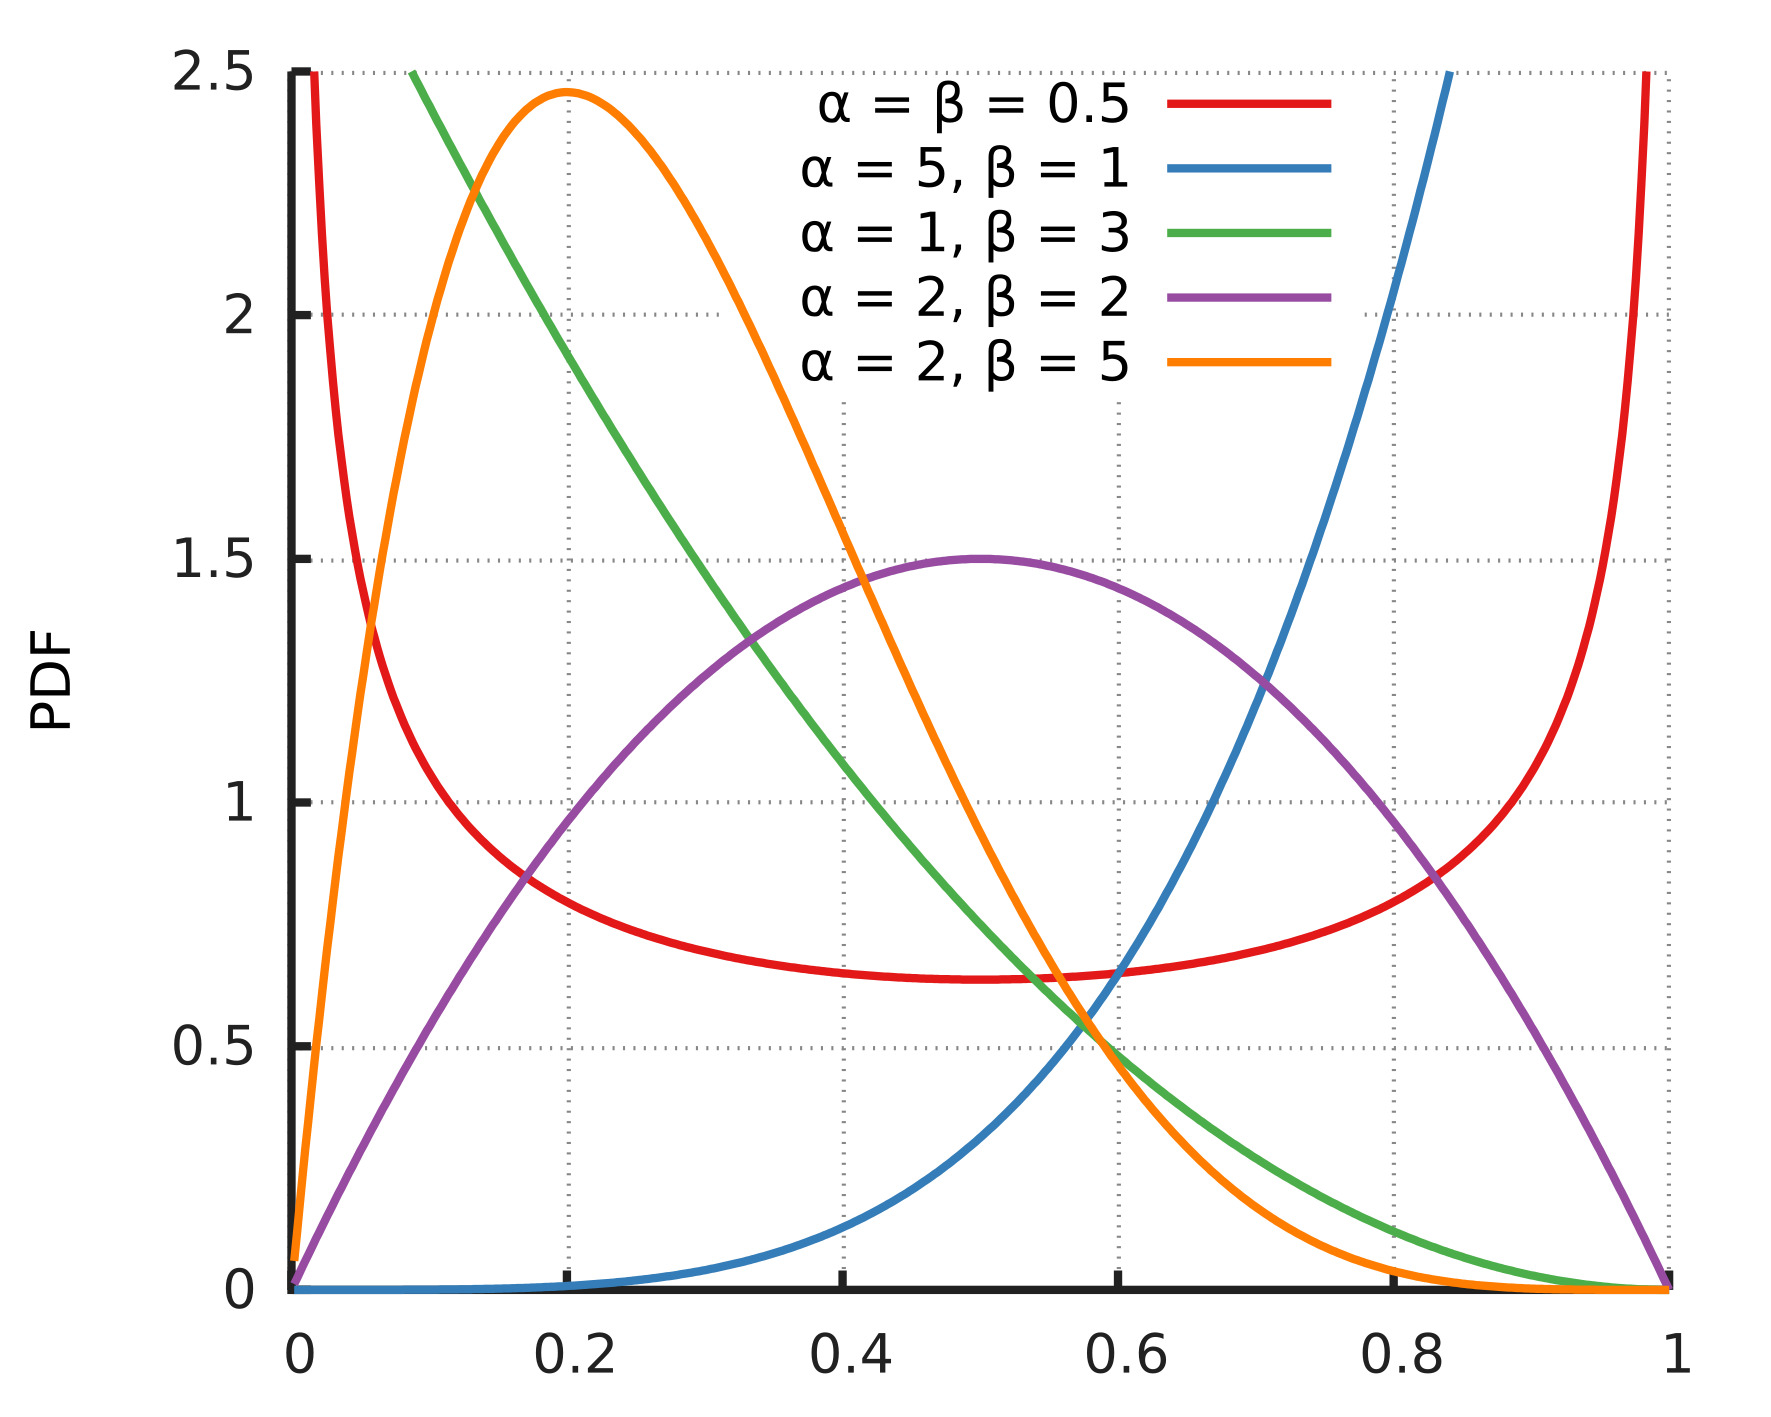
\includegraphics[width=\linewidth, height=4cm, keepaspectratio]{Pictures/distributions/Beta_distribution_pdf.jpg}
            \caption{Beta Distribution: PDF}
        \end{figure}
    \end{minipage}
    \hfill
    \begin{minipage}{0.49\linewidth}
        \begin{figure}[H]
            \centering
            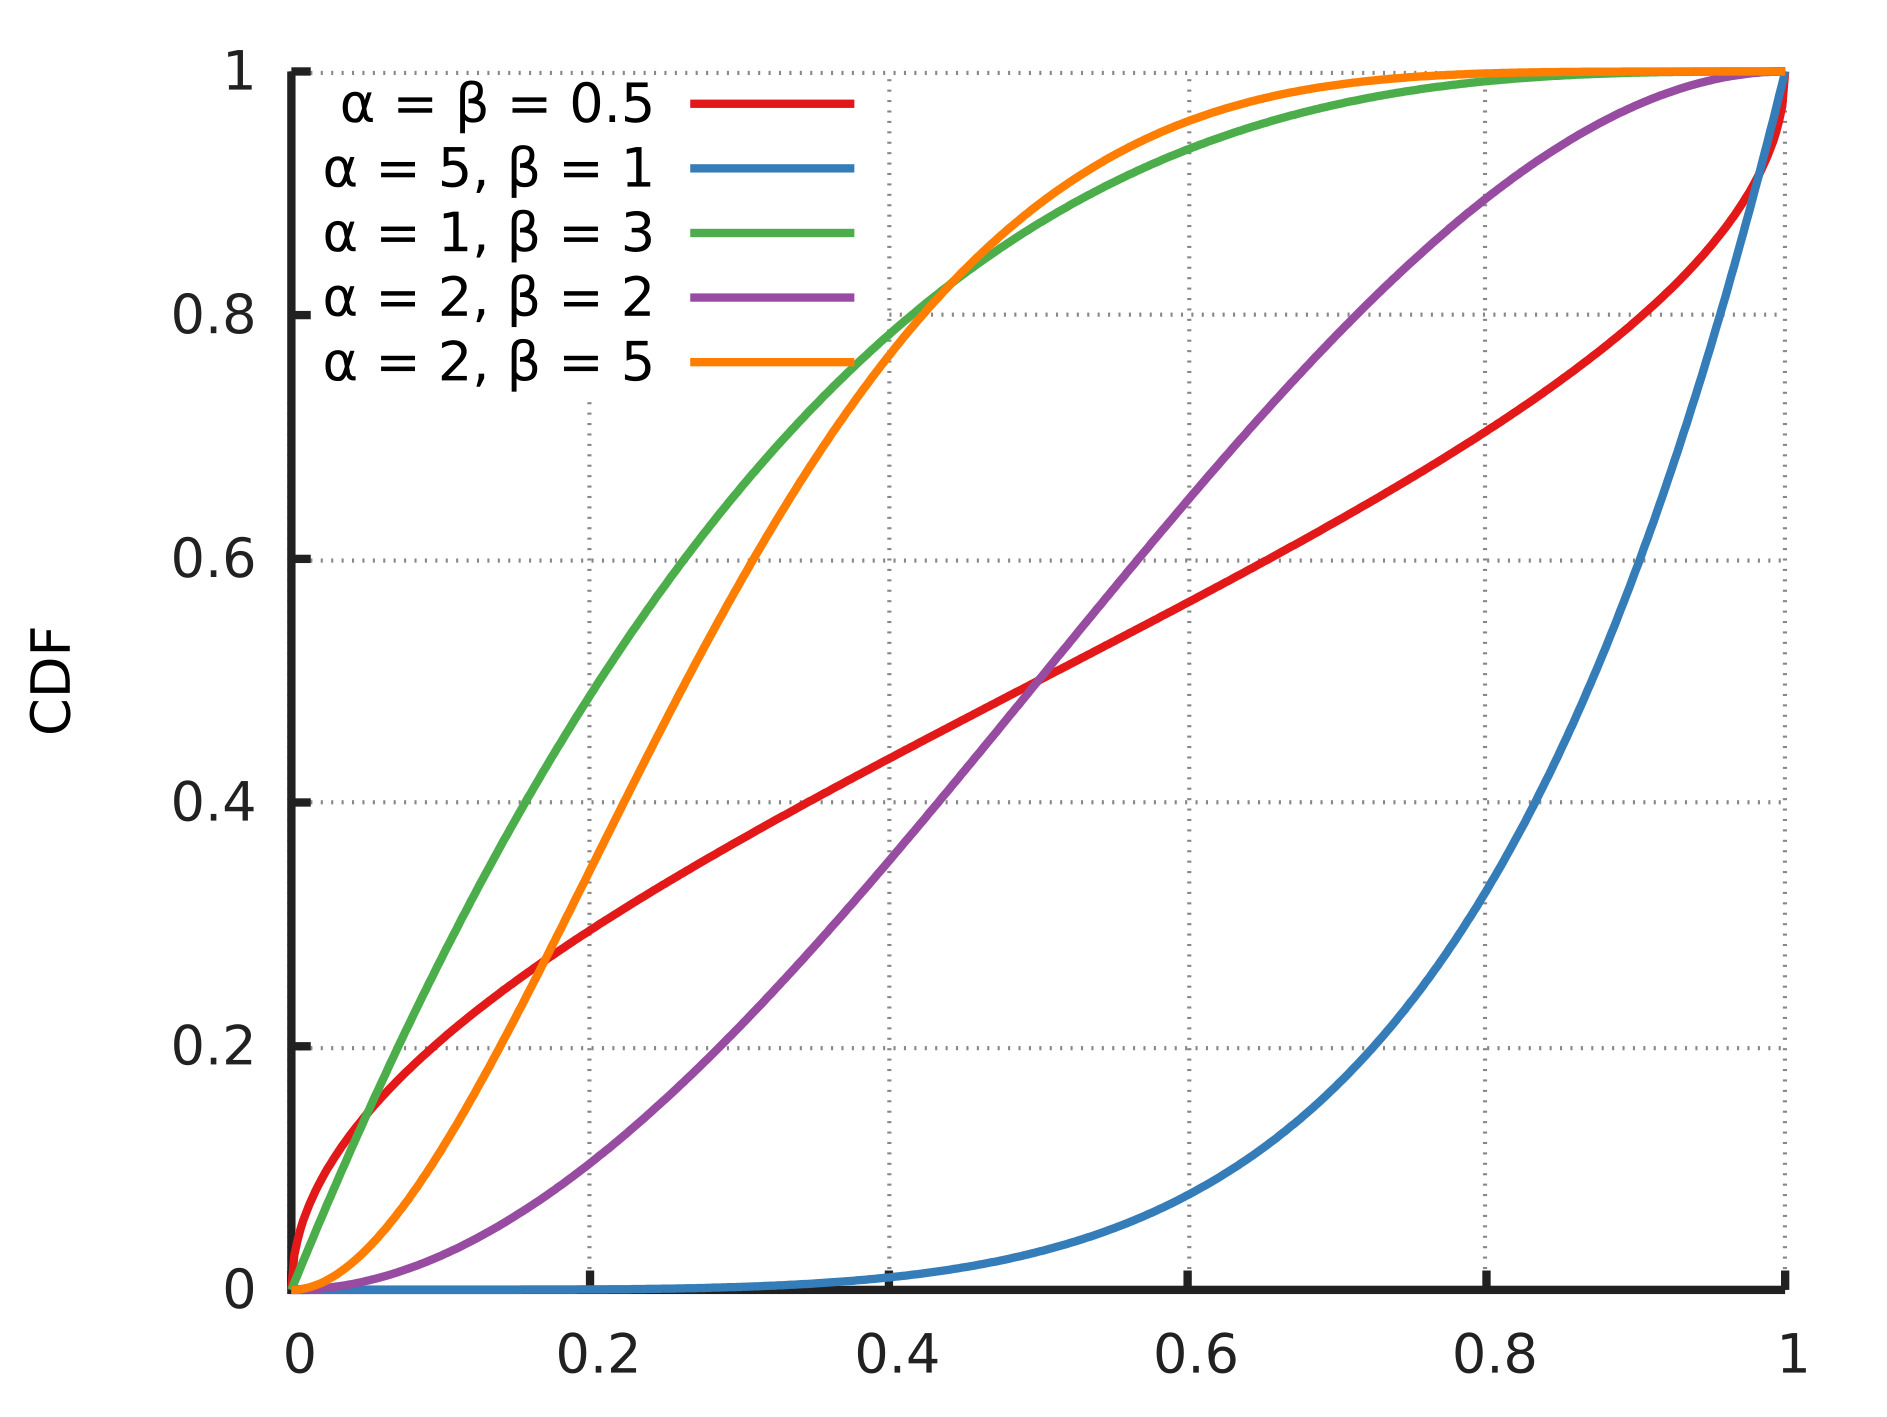
\includegraphics[width=\linewidth, height=4cm, keepaspectratio]{Pictures/distributions/Beta_distribution_cdf.jpg}
            \caption{Beta Distribution: CDF}
        \end{figure}
    \end{minipage}
\end{table}

\begin{alternateColorTable}
\renewcommand{\arraystretch}{2}
\begin{longtable}{|m{6cm}|p{9cm}|}
    \hline
    \tableHeaderRow
    \multicolumn{2}{|c|}{\textbf{Beta Distribution - Info} \cite{wiki/Beta_distribution}} \\
    \hline\endfirsthead

    \hline
    \tableHeaderRow
    \multicolumn{2}{|c|}{\textbf{Beta Distribution - Info - contd.} \cite{wiki/Beta_distribution}} \\
    \hline\endhead
    
    \hline\endfoot
    \hline\endlastfoot

    \textbf{Statistical parameters} & 
    \tableenumerate{
        \item $\alpha > 0$ shape (real)
        \item $\beta > 0$ shape (real)
    }
    \\[1ex] \hline
    
    \textbf{Support} &
    ${\displaystyle x\in [0,1]\!}$ or ${\displaystyle x\in (0,1)\!}$
    \\[1ex] \hline

    \textbf{Probability Density Function (PDF)} & 
    \tableenumerate{
        \item[] ${\displaystyle {\dfrac {x^{\alpha -1}(1-x)^{\beta -1}}{\mathrm {B} (\alpha ,\beta )}}\!}$
        
        \item[] where ${\displaystyle \mathrm {B} (\alpha ,\beta )={\dfrac {\Gamma (\alpha )\Gamma (\beta )}{\Gamma (\alpha +\beta )}}}$ and ${\displaystyle \Gamma }$ is the Gamma function.
    }
    \\[1ex] \hline
    
    \textbf{Cumulative distribution function (CDF)} & 
    ${\displaystyle I_{x}(\alpha ,\beta )\!}$
    \\[1ex] \hline

    \textbf{Mean} & 
    \tableenumerate{
        \item ${\displaystyle \operatorname {E} [X]={\dfrac {\alpha }{\alpha +\beta }}\!}$

        \item ${\displaystyle \operatorname {E} [\ln X]=\psi (\alpha )-\psi (\alpha +\beta )\!}$

        \item ${\displaystyle \operatorname {E} [X\,\ln X]={\dfrac {\alpha }{\alpha +\beta }}\,\left[\psi (\alpha +1)-\psi (\alpha +\beta +1)\right]\!}$

        \item[] where ${\displaystyle \psi }$ is the digamma function
    }
    \\[1ex] \hline

    \textbf{Median} & 
    ${\displaystyle {\begin{matrix}I_{\dfrac {1}{2}}^{[-1]}(\alpha ,\beta ){\text{ (in general) }}\\[0.5em]\approx {\dfrac {\alpha -{\dfrac {1}{3}}}{\alpha +\beta -{\dfrac {2}{3}}}}{\text{ for }}\alpha ,\beta >1\end{matrix}}}$
    \\[1ex] \hline

    \textbf{Mode} & 
    \tableenumerate{
        \item ${\displaystyle {\dfrac {\alpha -1}{\alpha +\beta -2}}\!}$ for $\alpha, \beta > 1$

        \item any value in ${\displaystyle (0,1)}$ for $\alpha, \beta = 1$

        \item $\dCurlyBrac{0, 1}$ (bimodal) for $\alpha, \beta < 1$

        \item $0$ for $\alpha \leq 1, \beta \geq 1, \alpha \neq \beta$

        \item $1$ for $\alpha \geq 1, \beta \leq 1, \alpha \neq \beta$
    }
    \\[1ex] \hline

    \textbf{Variance} &
    \tableenumerate{
        \item ${\displaystyle \operatorname {var} [X]={\dfrac {\alpha \beta }{(\alpha +\beta )^{2}(\alpha +\beta +1)}}\!}$

        \item ${\displaystyle \operatorname {var} [\ln X]=\psi _{1}(\alpha )-\psi _{1}(\alpha +\beta )\!}$
    }
    \\[1ex] \hline

    \textbf{Mean absolute deviation (MAD)} &
    \\[1ex] \hline

    \textbf{Skewness} &
    ${\displaystyle {\dfrac {2\,(\beta -\alpha ){\sqrt {\alpha +\beta +1}}}{(\alpha +\beta +2){\sqrt {\alpha \beta }}}}}$
    \\[1ex] \hline

    \textbf{Excess kurtosis} &
    ${\displaystyle {\dfrac {6[(\alpha -\beta )^{2}(\alpha +\beta +1)-\alpha \beta (\alpha +\beta +2)]}{\alpha \beta (\alpha +\beta +2)(\alpha +\beta +3)}}}$
    \\[1ex] \hline

    \textbf{Entropy} &
    ${\displaystyle {\begin{matrix}\ln \mathrm {B} (\alpha ,\beta )-(\alpha -1)\psi (\alpha )-(\beta -1)\psi (\beta )\\[0.5em]{}+(\alpha +\beta -2)\psi (\alpha +\beta )\end{matrix}}}$
    \\[1ex] \hline

    \textbf{Moment-generating function (MGF)} &
    ${\displaystyle 1+\sum _{k=1}^{\infty }\left(\prod _{r=0}^{k-1}{\dfrac {\alpha +r}{\alpha +\beta +r}}\right){\dfrac {t^{k}}{k!}}}$
    \\[1ex] \hline

    \textbf{Characteristic function (CF)} &
    ${\displaystyle {}_{1}F_{1}(\alpha ;\alpha +\beta ;i\,t)\!}$ (see Confluent hypergeometric function)
    \\[1ex] \hline

    \textbf{Fisher information} &
    ${\displaystyle {\begin{bmatrix}\operatorname {var} [\ln X]&\operatorname {cov} [\ln X,\ln(1-X)]\\\operatorname {cov} [\ln X,\ln(1-X)]&\operatorname {var} [\ln(1-X)]\end{bmatrix}}}$
    \\[1ex] \hline

    \textbf{Method of moments} &
    \tableenumerate{
        \item ${\displaystyle \alpha =\left({\dfrac {E[X](1-E[X])}{V[X]}}-1\right)E[X]}$
        \vspace{0.1cm}

        \item ${\displaystyle \beta =\left({\dfrac {E[X](1-E[X])}{V[X]}}-1\right)(1-E[X])}$
        \vspace{0.2cm}
    }
    \\[2ex] \hline

\end{longtable}
\renewcommand{\arraystretch}{1}
\end{alternateColorTable}

\begin{enumerate}
    \item considered a \textbf{conjugate prior distribution}

    \item if $\alpha = 1$ and $\beta = 1$, the resulting beta distribution function is actually a \textbf{uniform distribution} function on $[0, 1]$ \cite{ism-1}

    \item For $\alpha, \beta < 1$, we get a \textbf{bimodal distribution} with spikes at $0$ and $1$. \cite{mfml-1}

    \item For $\alpha, \beta > 1$, the distribution is \textbf{unimodal}. \cite{mfml-1}

    \item For $\alpha, \beta > 1$ and $\alpha = \beta$, the distribution is \textbf{unimodal, symmetric}, and centered in the interval $[0, 1]$, i.e., the mode/mean is at $1/2$. \cite{mfml-1}
\end{enumerate}

\section{Bayesian Analysis \cite{ism-1}} \label{Beta Distribution: Bayesian Analysis}

\begin{enumerate}
    \item Posterior: \cite{ism-1}
    \begin{align*}
         f(\theta|x) 
         &\propto p(x|\theta) f (\theta) \\
         &= \theta^{\sum^{n}_{i=1} x_i} 
            (1 - \theta)^{n - \sum^{n}_{i=1} x_i}
            \dfrac{\Gamma (\alpha + \beta)}{\Gamma (\alpha)\Gamma (\beta)}
            \theta^{\alpha-1} (1 - \theta)^{\beta-1} \\
        &\propto \theta^{(\alpha + \sum^{n}_{i=1} x_i)-1} 
            (1-\theta)^{(\beta + n - \sum^{n}_{i=1} x_i)-1} 
    \end{align*}

    \begin{enumerate}
        \item[] posterior $f (\theta|D)$ is proportional to the density of a $beta(\alpha', \beta')$ distribution:
        \begin{enumerate}
            \item $\alpha' = \alpha + \dsum^{n}_{i=1} xi$

            \item $\beta' = \beta + n - \dsum^{n}_{i=1} xi$
        
        \end{enumerate}

    \end{enumerate}

    \item Prior:
    \begin{enumerate}
        \item $\alpha$ specifies the a-priori number of \textbf{successes}

        \item $\beta$ specifies the a-priori number of \textbf{failures}

    \end{enumerate}

\end{enumerate}







